%%%%%%%%%%%%%%%%%%%%%%%%%%%%%%%%%%%%%%%%%
% Beamer Presentation
% LaTeX Template
% Version 1.0 (10/11/12)
%
% This template has been downloaded from:
% http://www.LaTeXTemplates.com
%
% License:
% CC BY-NC-SA 3.0 (http://creativecommons.org/licenses/by-nc-sa/3.0/)
%
%%%%%%%%%%%%%%%%%%%%%%%%%%%%%%%%%%%%%%%%%

%----------------------------------------------------------------------------------------
%	PACKAGES AND THEMES
%----------------------------------------------------------------------------------------

\documentclass{beamer}

\mode<presentation> {

% The Beamer class comes with a number of default slide themes
% which change the colors and layouts of slides. Below this is a list
% of all the themes, uncomment each in turn to see what they look like.

%\usetheme{default}
%\usetheme{AnnArbor}
%\usetheme{Antibes}
%\usetheme{Bergen}
%\usetheme{Berkeley}
%\usetheme{Berlin}
%\usetheme{Boadilla}
%\usetheme{CambridgeUS} %Color rojo, me gusta
%\usetheme{Copenhagen} %Ta bueno
\usetheme{Darmstadt} % Este es el 1er candidato
%\usetheme{Dresden} % Es lindo y parecido al de arriba
%\usetheme{Frankfurt}
%\usetheme{Goettingen}
%\usetheme{Hannover}
%\usetheme{Ilmenau}
%\usetheme{JuanLesPins}
%\usetheme{Luebeck}
%\usetheme{Madrid}
%\usetheme{Malmoe}
%\usetheme{Marburg}
%\usetheme{Montpellier}
%\usetheme{PaloAlto}
%\usetheme{Pittsburgh}
%\usetheme{Rochester}
%\usetheme{Singapore}
%\usetheme{Szeged}
%\usetheme{Warsaw}

% As well as themes, the Beamer class has a number of color themes
% for any slide theme. Uncomment each of these in turn to see how it
% changes the colors of your current slide theme.

%\usecolortheme{albatross}
%\usecolortheme{beaver}
%\usecolortheme{beetle}
%\usecolortheme{crane}
%\usecolortheme{dolphin}
%\usecolortheme{dove}
%\usecolortheme{fly}
%\usecolortheme{lily}
%\usecolortheme{orchid}
%\usecolortheme{rose}
%\usecolortheme{seagull}
%\usecolortheme{seahorse}
%\usecolortheme{whale}
%\usecolortheme{wolverine}

%\setbeamertemplate{footline} % To remove the footer line in all slides uncomment this line
%\setbeamertemplate{footline}[page number] % To replace the footer line in all slides with a simple slide count uncomment this line

%\setbeamertemplate{navigation symbols}{} % To remove the navigation symbols from the bottom of all slides uncomment this line
}

\usepackage{graphicx} % Allows including images
\usepackage{booktabs} % Allows the use of \toprule, \midrule and \bottomrule in tables
\usepackage{listings}
%\usepackage{url}
\usepackage{hyperref}
\usepackage[spanish]{babel}
\usepackage[utf8]{inputenc}
%----------------------------------------------------------------------------------------
%	TITLE PAGE
%----------------------------------------------------------------------------------------

\title[Flujo Analógico]{Instalación y Configuración de un Flujo de Diseño Analógico} % The short title appears at the bottom of every slide, the full title is only on the title page

\author{Leandro Marsó} % Your name
\institute[] % Your institution as it will appear on the bottom of every slide, may be shorthand to save space
{
Córdoba\\ % Your institution for the title page
\medskip
\textit{elleandro@gmail.com} % Your email address
}
\date{\today} % Date, can be changed to a custom date

\begin{document}


\lstset{
basicstyle=\ttfamily,                   % Code font, Examples: \footnotesize, \ttfamily
frame=none,                             % A frame around the code
tabsize=2,                              % Default tab size
captionpos=b,                           % Caption-position = bottom
breaklines=false,                        % Automatic line breaking?
breakatwhitespace=false,                % Automatic breaks only at whitespace?
showspaces=false,                       % Dont make spaces visible
showtabs=false,                         % Dont make tabls visible
showstringspaces=false,
commentstyle=\color{red},
keywordstyle=\color{blue},
}


\begin{frame}
\titlepage % Print the title page as the first slide
\end{frame}

\begin{frame}
\frametitle{Contenido} % Table of contents slide, comment this block out to remove it
\tableofcontents % Throughout your presentation, if you choose to use \section{} and \subsection{} commands, these will automatically be printed on this slide as an overview of your presentation
\end{frame}

%----------------------------------------------------------------------------------------
%	PRESENTATION SLIDES
%----------------------------------------------------------------------------------------
\section{¿Qué es el Software Libre?}
\begin{frame}
\frametitle{Definición de software libre}
«Software libre» es el software que respeta la libertad de los usuarios y la comunidad. A grandes rasgos, significa que los usuarios tienen la libertad de ejecutar, copiar, distribuir, estudiar, modificar y mejorar el software. Es decir, el «software libre» es una cuestión de libertad, no de precio.

\end{frame}
%------------------------------------------------
\begin{frame}
\frametitle{Las cuatro libertades del Software Libre}
Un programa es software libre si los usuarios tienen las cuatro libertades esenciales:
\begin{itemize}
\item La libertad de ejecutar el programa como se desea, con cualquier propósito (libertad 0).
\item La libertad de estudiar cómo funciona el programa, y cambiarlo para que haga lo que usted quiera (libertad 1). El acceso al código fuente es una condición necesaria para ello.
\item La libertad de redistribuir copias para ayudar a su prójimo (libertad 2).
\item La libertad de distribuir copias de sus versiones modificadas a terceros (libertad 3). Esto le permite ofrecer a toda la comunidad la oportunidad de beneficiarse de las modificaciones. El acceso al código fuente es una condición necesaria para ello.
\end{itemize}
\end{frame}

\section{Instalación} % Sections can be created in order to organize your presentation into discrete blocks, all sections and subsections are automatically printed in the table of contents as an overview of the talk

%------------------------------------------------

\begin{frame}[fragile]
\subsection{Instalacíon de paquetes necesarios } % A subsection can be created just before a set of slides with a common theme to further break down your presentation into chunks

\frametitle{Instalación del JDK de Java, gnucap y otras herramientas}

\noindent Desde una consola:
\begin{lstlisting}[language=bash]
 # Acceder a privilegios de root
 su
 apt-get install openjdk-6-jdk gnucap \
 perl python-matplotlib
 # Abandonar los privilegios de root
 exit
\end{lstlisting}
\end{frame}
%----------------------------------------------------

\subsection{Electric}
\begin{frame}[fragile]
\frametitle{Descargar Electric 9.05}

\noindent Desde la consola:
\begin{scriptsize}
\begin{lstlisting}[language=bash]
  mkdir -p ~/aflow/bin # Creo un directorio en mi home
  cd ~/aflow/bin	      # Cambio al directorio creado
  wget ftp://ftp.gnu.org/pub/gnu/electric/electric-9.05.jar
\end{lstlisting}
\end{scriptsize}

O bien desde el navegador ir a:

 \url{http://www.staticfreesoft.com/productsFree.html}

y descargar cualquiera de las dos opciones disponibles (binario y código fuente o binario solamente):
\begin{figure}
\includegraphics[width=0.8\linewidth]{figuras/downloadElectric.png}
\end{figure}
Descargar también algunos plug-ins:
\begin{scriptsize}
\begin{lstlisting}[language=bash]
  wget http://www.staticfreesoft.com/electricSFS-9.05.jar
\end{lstlisting}
\end{scriptsize}
\end{frame}


%------------------------------------------------
\begin{frame}[fragile]
\frametitle{Crear acceso directo a Electric}
Desde una consola hacer:
\begin{tiny}
\begin{lstlisting}[language=bash]
 echo "alias electric='java -classpath ~/aflow/bin/electric-9.05.jar:\
 ~/aflow/bin/electricSFS-9.05.jar com.sun.electric.Launcher &'" >> ~/.bashrc
\end{lstlisting}

\end{tiny}

\end{frame}

%------------------------------------------------
\begin{frame}[fragile]
\section{Configuración}
\frametitle{General}

\noindent Abrimos la configuración en file $\rightarrow$ Preferences...

\begin{figure}
\includegraphics[width=0.6\linewidth]{figuras/configuracionElectric-1.png}
\end{figure}
\end{frame}


%------------------------------------------------
\begin{frame}
\frametitle{Electric}

\noindent En Categories $\rightarrow$ General $\rightarrow$ General editamos donde está recuadrado y hacemos click en Apply 

\begin{figure}
\includegraphics[width=0.55\linewidth]{figuras/configuracionElectric-2.png}
\end{figure}
\end{frame}

%------------------------------------------------
\begin{frame}[fragile]
\subsection{SPICE}
\frametitle{Electric - Simulador SPICE}

\noindent En Tools $\rightarrow$ Spice/CDL editamos donde está recuadrado y hacemos click en Apply 

\begin{figure}
\includegraphics[width=0.6\linewidth]{figuras/configuracionElectric-3.png}
\end{figure}
\end{frame}

%------------------------------------------------
\begin{frame}[fragile]
\frametitle{Electric - Parámetros del modelo SPICE}

Definimos el archivo que contiene los parámetros del modelo de simulación de los transistores.
En nuestro caso elegimos del sitio de \href{https://www.mosis.com/pages/design/flows/design-flow-scmos-kits}{MOSIS} el proceso \href{https://www.mosis.com/rep/vendors/tsmc-035/v01c_mm_non_epi-params.txt}{TSMC $0.35~\textrm{um}$}.
A este archivo hay que comentar\footnote{En SPICE el caracter para comentar es el asterisco}  o borrar todo el texto hasta la línea (inclusive):

\begin{scriptsize}
\verb.SPICE 3f5 Level 8, Star-HSPICE Level 49, UTMOST Level 8.
\end{scriptsize}

Y finalmente las líneas:

\begin{scriptsize}
\verb#.MODEL CMOSN NMOS#
\end{scriptsize} cambiar por \begin{scriptsize}\verb#.MODEL N NMOS# 

\verb#.MODEL CMOSP PMOS#\end{scriptsize} cambiar por \begin{scriptsize}\verb#.MODEL P PMOS# \end{scriptsize}

Guardamos el archivo en un directorio apropiado y desde Electric indicamos su ubicación,
como muestra la figura:
\begin{figure}
\includegraphics[width=0.6\linewidth]{figuras/configuracionElectric-4.png}
\end{figure}

\end{frame}

%------------------------------------------------
\begin{frame}
\subsection{Tecnología}
\frametitle{Electric - Tecnología}

\noindent En Technology $\rightarrow$ Technology editamos donde está recuadrado:
\begin{figure}
\includegraphics[width=0.7\linewidth]{figuras/configuracionElectric-5.png}
\end{figure}
\end{frame}

%------------------------------------------------
\begin{frame}
\subsection{Lambda}
\frametitle{Electric - Lambda}

Del documento sobre \href{https://www.mosis.com/files/scmos/scmos.pdf}{MOSIS Scalable CMOS (SCMOS)} elegimos las reglas SCN4ME\_SUBM, que determinan el valor de Lambda sea 0.2um para 0.35um. Esta información también se encuentra en la documentación del proceso del sitio de \href{https://www.mosis.com/vendors/view/tsmc/035}{MOSIS}: 
\begin{figure}
\includegraphics[width=0.7\linewidth]{figuras/configuracionElectric-6.png}
\end{figure}
\end{frame}

 
%------------------------------------------------
\begin{frame}
\frametitle{Electric - Lambda}
En Technology  $\rightarrow$ Scale modificamos el valor de Lambda:
\begin{figure}
\includegraphics[width=0.7\linewidth]{figuras/configuracionElectric-7.png}
\end{figure}
\end{frame}


%------------------------------------------------
\begin{frame}
\subsection{DRC}
\frametitle{Electric - Design Rules}
En Technology  $\rightarrow$ Design Rules accedemos a la configuración de las reglas de diseño, según en el documento \href{https://www.mosis.com/files/scmos/scmos.pdf}{SCMOS} :
\begin{figure}
\includegraphics[width=0.7\linewidth]{figuras/configuracionElectric-8.png}
\end{figure}
\end{frame}


%------------------------------------------------
\begin{frame}
\frametitle{Electric - Design Rules - Ejemplos}
\begin{columns}[t] % The "c" option specifies centered vertical alignment while the "t" option is used for top vertical alignment
\column{.6\textwidth} % Left column and width
\textbf{DRC Electric}
\begin{figure}
\includegraphics[width=0.99\linewidth]{figuras/configuracionElectric-8b.png}
\end{figure}
\column{.4\textwidth} % Right column and width
\textbf{Especificación de DRC}
\begin{figure}
\includegraphics[width=0.99\linewidth]{figuras/configuracionElectric-9.png}
\end{figure}
\end{columns}
\end{frame}

%------------------------------------------------
\begin{frame}
\frametitle{Electric - Design Rules - Ejemplos}
\begin{columns}[t] % The "c" option specifies centered vertical alignment while the "t" option is used for top vertical alignment
\column{.6\textwidth} % Left column and width
\textbf{DRC Electric}
\begin{figure}
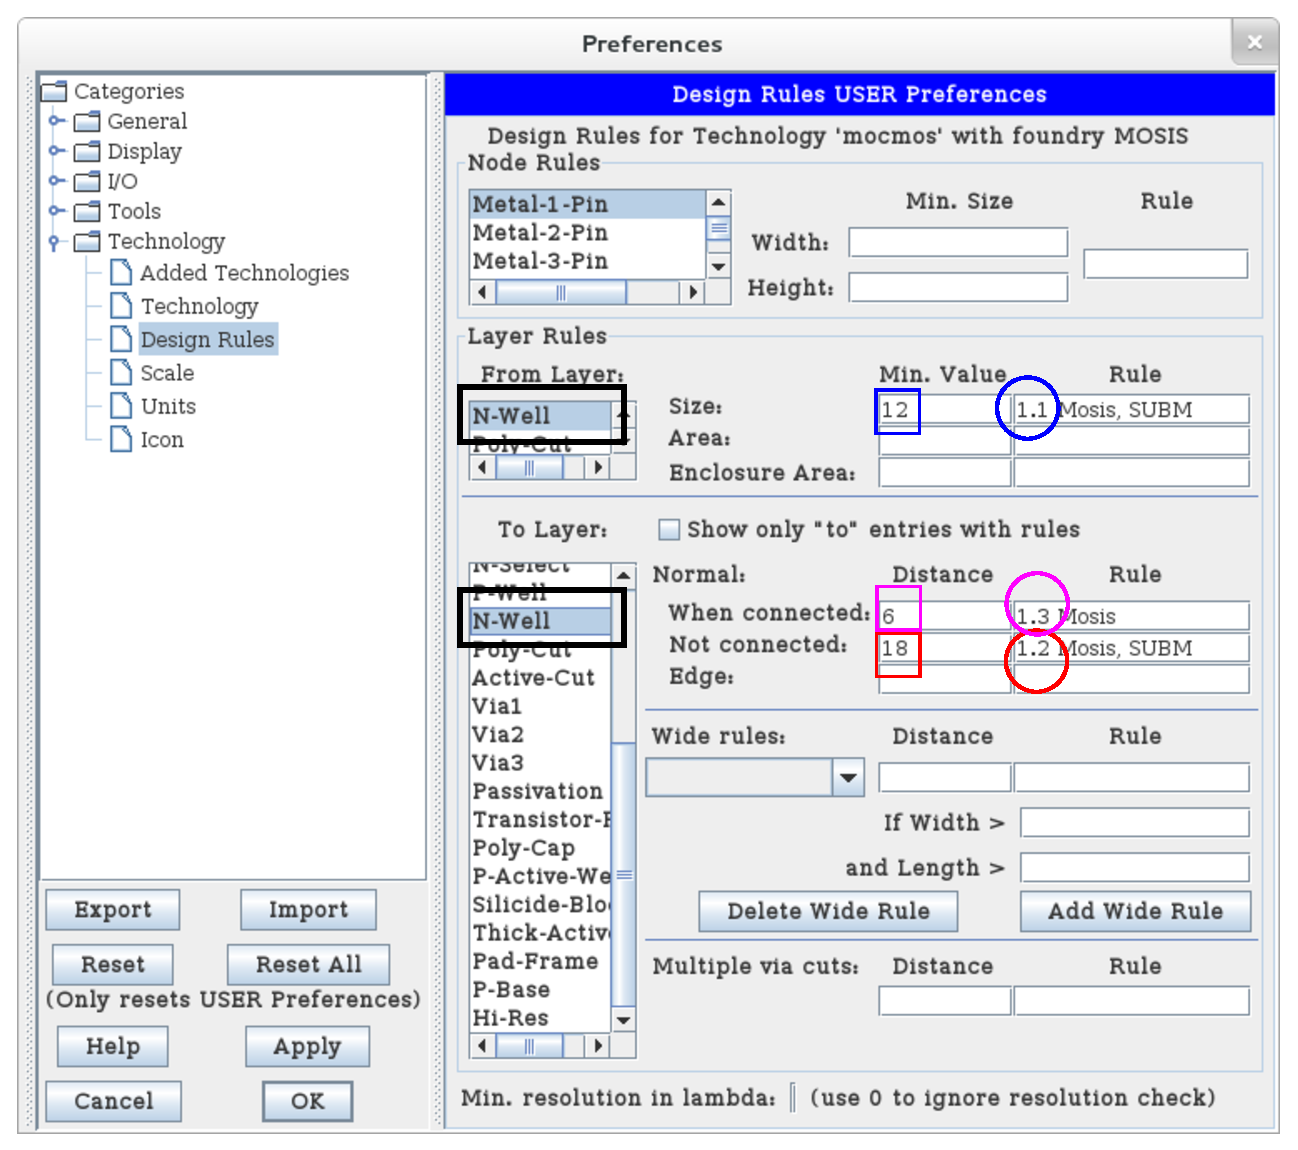
\includegraphics[width=0.99\linewidth]{figuras/configuracionElectric-10B.eps}
\end{figure}
\column{.55\textwidth} % Right column and width
\textbf{Especificación de DRC}
\begin{figure}
%\includegraphics[width=1.00\linewidth]{figuras/scmos.eps}
\includegraphics[width=1.00\linewidth]{figuras/scmos-eps-converted-to.pdf}
\end{figure}

\end{columns}
\end{frame}

%------------------------------------------------
\begin{frame}[fragile]
\frametitle{Electric - Extracción de Parásitos}
\begin{columns}[t] % The "c" option specifies centered vertical alignment while the "t" option is used for top vertical alignment
\column{.6\textwidth} % Left column and width
\textbf{Configuración en Electric}
\begin{figure}
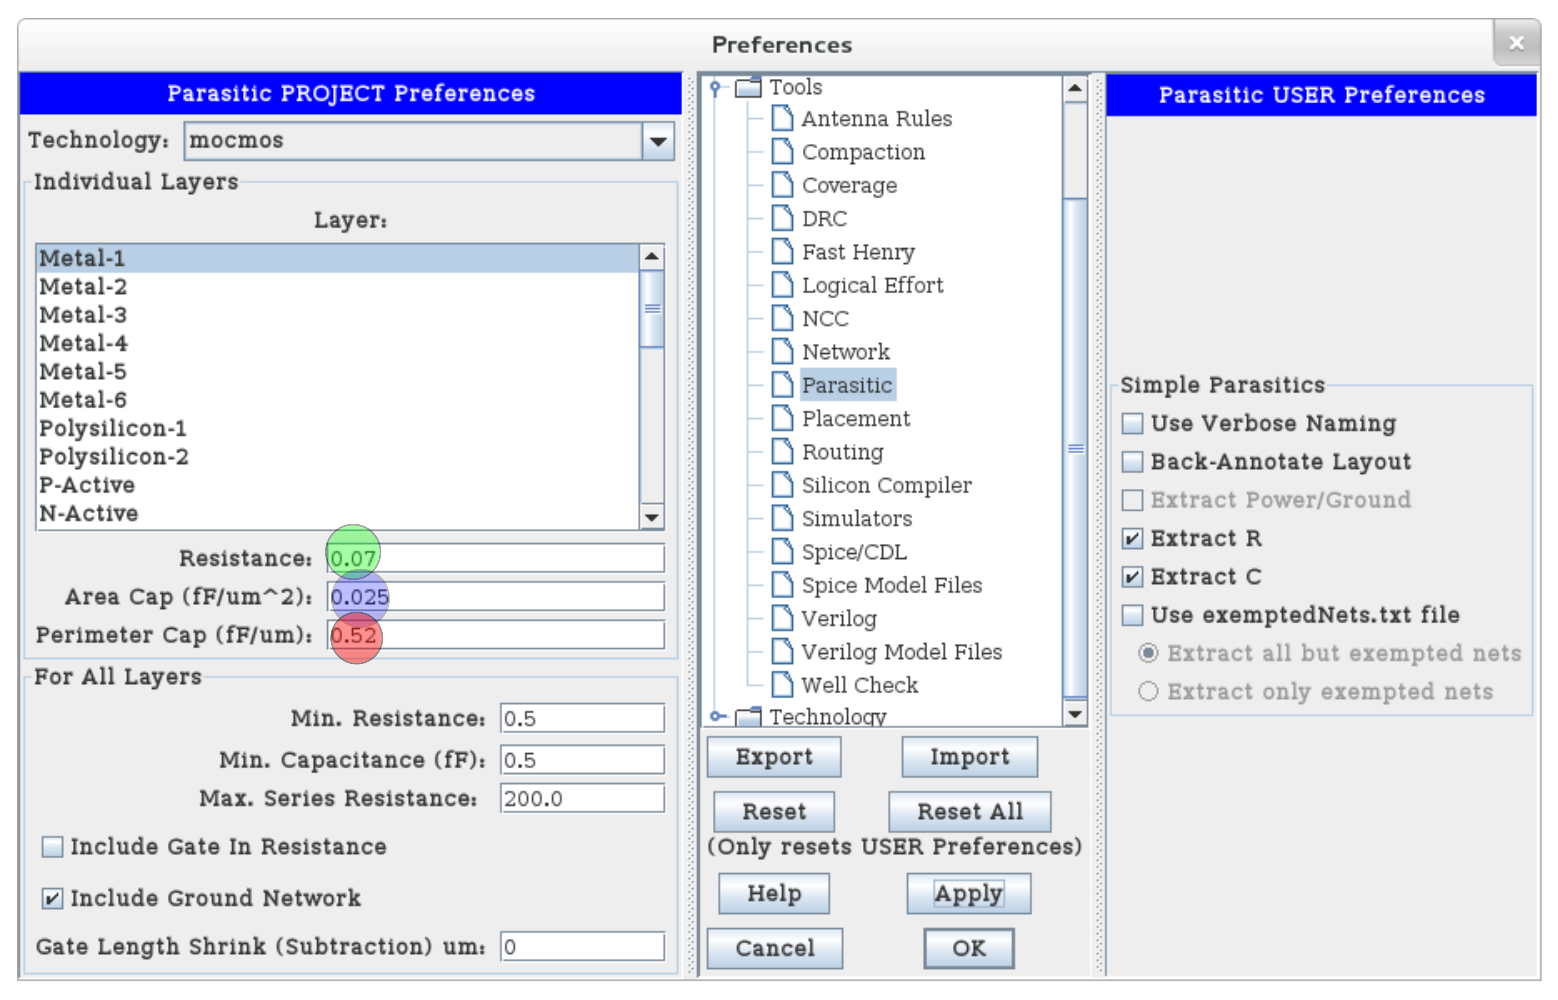
\includegraphics[width=0.99\linewidth]{figuras/configuracionElectric-11a.eps}
\end{figure}

\column{.55\textwidth} % Right column and width
\textbf{Info sobre parásitos brindado por el fabricante}
\begin{figure}
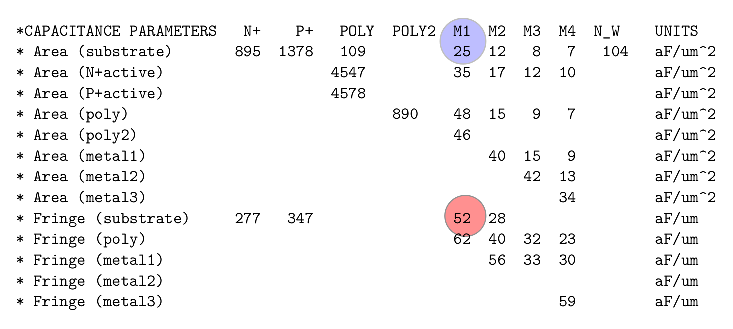
\includegraphics[width=1\linewidth]{figuras/configuracionElectric-11b.eps}
\end{figure}
\vspace{-0.8cm}
\begin{figure}
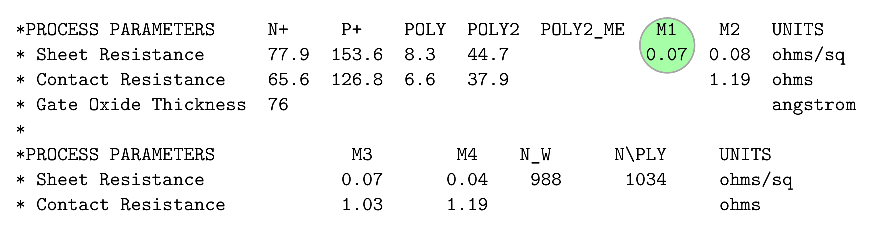
\includegraphics[width=1\linewidth]{figuras/configuracionElectric-11c.eps}
\end{figure}


\end{columns}
\end{frame}

%------------------------------------------------
\begin{frame}
\frametitle{Electric - Extracción de Parásitos - Advertencia}
\begin{Huge}\centerline{Advertencia}
\end{Huge}

La herramienta de extracción de elementos parásitos de \textbf{Electric} es muy limitada, ya que no extrae las capacidades entre las distintas capas. La extracción que realiza es sólo entre las distintas capas y el sustrato. Por lo tanto, hemos de utilizar otra herramienta para este propósito cuando realizamos un diseño real. Con el fin de simplificar esta presentación, utilizaremos la herramienta de extracción de \textbf{Electric}.  
\end{frame}


%------------------------------------------------
%\section{Edición de Circuitos}
%\begin{frame}
%\subsection{Esquemáticos}
%
%\end{frame}
%
%
%%------------------------------------------------
%
%
%\begin{frame}
%\frametitle{Blocks of Highlighted Text}
%\begin{block}{Block 1}
%Lorem ipsum dolor sit amet, consectetur adipiscing elit. Integer lectus nisl, ultricies in feugiat rutrum, porttitor sit amet augue. Aliquam ut tortor mauris. Sed volutpat ante purus, quis accumsan dolor.
%\end{block}
%
%\begin{block}{Block 2}
%Pellentesque sed tellus purus. Class aptent taciti sociosqu ad litora torquent per conubia nostra, per inceptos himenaeos. Vestibulum quis magna at risus dictum tempor eu vitae velit.
%\end{block}
%
%\begin{block}{Block 3}
%Suspendisse tincidunt sagittis gravida. Curabitur condimentum, enim sed venenatis rutrum, ipsum neque consectetur orci, sed blandit justo nisi ac lacus.
%\end{block}
%\end{frame}
%
%%------------------------------------------------
%
%\begin{frame}
%\frametitle{Multiple Columns}
%\begin{columns}[c] % The "c" option specifies centered vertical alignment while the "t" option is used for top vertical alignment
%
%\column{.45\textwidth} % Left column and width
%\textbf{Heading}
%\begin{enumerate}
%\item Statement
%\item Explanation
%\item Example
%\end{enumerate}
%
%\column{.5\textwidth} % Right column and width
%Lorem ipsum dolor sit amet, consectetur adipiscing elit. Integer lectus nisl, ultricies in feugiat rutrum, porttitor sit amet augue. Aliquam ut tortor mauris. Sed volutpat ante purus, quis accumsan dolor.
%
%\end{columns}
%\end{frame}
%
%%------------------------------------------------
%\section{Second Section}
%%------------------------------------------------
%
%\begin{frame}
%\frametitle{Table}
%\begin{table}
%\begin{tabular}{l l l}
%\toprule
%\textbf{Treatments} & \textbf{Response 1} & \textbf{Response 2}\\
%\midrule
%Treatment 1 & 0.0003262 & 0.562 \\
%Treatment 2 & 0.0015681 & 0.910 \\
%Treatment 3 & 0.0009271 & 0.296 \\
%\bottomrule
%\end{tabular}
%\caption{Table caption}
%\end{table}
%\end{frame}
%
%%------------------------------------------------
%
%\begin{frame}
%\frametitle{Theorem}
%\begin{theorem}[Mass--energy equivalence]
%$E = mc^2$
%\end{theorem}
%\end{frame}
%
%%------------------------------------------------
%
%\begin{frame}[fragile] % Need to use the fragile option when verbatim is used in the slide
%\frametitle{Verbatim}
%\begin{example}[Theorem Slide Code]
%\begin{verbatim}
%\begin{frame}
%\frametitle{Theorem}
%\begin{theorem}[Mass--energy equivalence]
%$E = mc^2$
%\end{theorem}
%\end{frame}\end{verbatim}
%\end{example}
%\end{frame}
%
%%------------------------------------------------
%
%\begin{frame}
%\frametitle{Figure}
%Uncomment the code on this slide to include your own image from the same directory as the template .TeX file.
%%\begin{figure}
%%\includegraphics[width=0.8\linewidth]{test}
%%\end{figure}
%\end{frame}
%
%%------------------------------------------------
%
%\begin{frame}[fragile] % Need to use the fragile option when verbatim is used in the slide
%\frametitle{Citation}
%An example of the \verb|\cite| command to cite within the presentation:\\~
%
%This statement requires citation \cite{p1}.
%\end{frame}
%
%%------------------------------------------------
%
%\begin{frame}
%\frametitle{References}
%\footnotesize{
%\begin{thebibliography}{99} % Beamer does not support BibTeX so references must be inserted manually as below
%\bibitem[Smith, 2012]{p1} John Smith (2012)
%\newblock Title of the publication
%\newblock \emph{Journal Name} 12(3), 45 -- 678.
%\end{thebibliography}
%}
%\end{frame}
%
%%------------------------------------------------
%
\begin{frame}
\Huge{\centerline{Fin}}
\end{frame}

%----------------------------------------------------------------------------------------

\end{document} 
